\documentclass[12pt]{article}
\usepackage{graphicx}

\usepackage{tikz}
\usetikzlibrary{}

\begin{document}

\section*{Simple node styles}

Try out the \textbackslash{}node commands to (roughly) replicate these nodes
\vspace{1em}

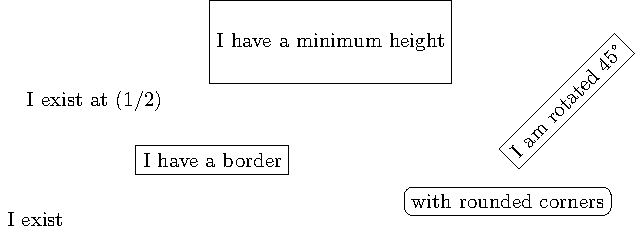
\includegraphics{_img_src/00_simple_node.pdf}

\vspace{1em}
\hrule 
\vspace{1em}

%%%%%%%%%%%%%%%%%%%%%
% Add your code here
%%%%%%%%%%%%%%%%%%%%%
\begin{tikzpicture}
    
\end{tikzpicture}

%-------------------------------------------------------

\pagebreak
\section{Simple node positioning}

Use the anchors and the relative positioning arguments to get similar results!
\vspace{1em}

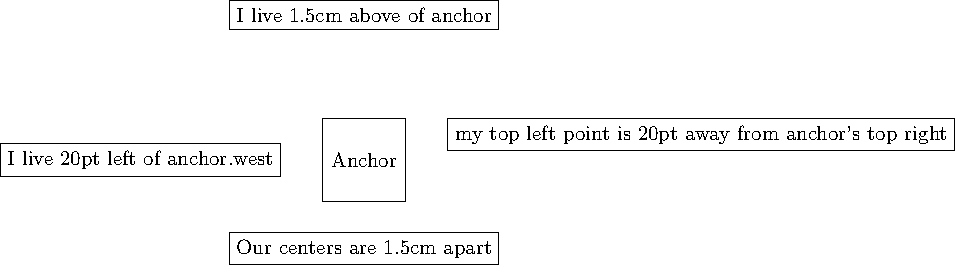
\includegraphics{_img_src/01_node_positioning.pdf}

\vspace{1em}
\hrule 
\vspace{1em}

%%%%%%%%%%%%%%%%%%%%%
% Add your code here
%%%%%%%%%%%%%%%%%%%%%
\begin{tikzpicture}
    
\end{tikzpicture}

%-------------------------------------------------------

\pagebreak
\section{Shapes and colors make things look nice}

Now you know the drill.
\vspace{1em}

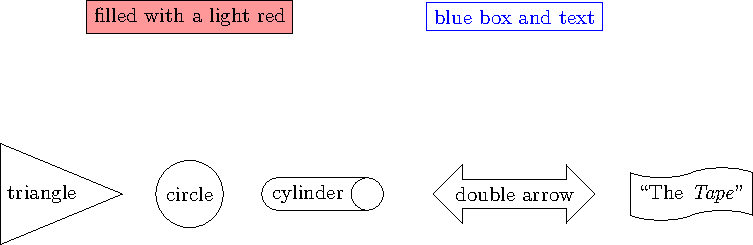
\includegraphics{_img_src/02_node_shapes_colors.pdf}

\vspace{1em}
\hrule 
\vspace{1em}

%%%%%%%%%%%%%%%%%%%%%
% Add your code here
%%%%%%%%%%%%%%%%%%%%%
\begin{tikzpicture}
    
\end{tikzpicture}

\end{document}